\documentclass[13pt, t]{beamer}
% Presento style file
\usepackage{config/presento}

% custom command and packages
% custom packages
\usepackage{textpos}
\setlength{\TPHorizModule}{1cm}
\setlength{\TPVertModule}{1cm}

\newcommand\crule[1][black]{\textcolor{#1}{\rule{2cm}{2cm}}}



\usepackage{color, colortbl}

\title{\Large \hspace{-0.5cm} Жестовая лингвистика}
\author[shortname]{Аня Клезович, Гарик Мороз}
\institute[shortinst]{Лаборатория языковой конвергенции, НИУ ВШЭ, Москва}
\date{\begin{center} 24 июля 2019 \bigskip \\ {{\color{colorblue} \href{www.letnyayashkola.org/}{\large Летняя Школа}}\\ \vfill Презентация доступна здесь: {\large \href{https://tinyurl.com/yxbkl3ke}{tinyurl.com/yxbkl3ke}}} \end{center}}

\begin{document}

\begin{frame}[plain]
\maketitle
\end{frame}

\section{Введение} % Гарик

\begin{frame}{Мифы про жестовые языки:}
\begin{itemize}
    \item ЖЯ не один (карта всех ЖЯ из lingtypology)
    \item жестикуляция не ЖЯ
    \item ЖЯ --- отдельный язык, хоть и с кучей заимствований из звучащего
    \item ЖЯ vs калькирующая речь (якобы сурдопереводчики из 90ых)
    \item глухонемые
\end{itemize}
\end{frame}

\section{История изучения} % Аня

\section{Граматические оссобенности РЖЯ} % Гарик

\section{Иконичность и одновременность} % Аня

\section{Фонетика и фонология} % Гарик

\section{Автоматическое распознавание ЖЯ} % Аня

\section{Песня, стихи и т. п.} % Гарик и Аня

\begin{frame}{yyy}
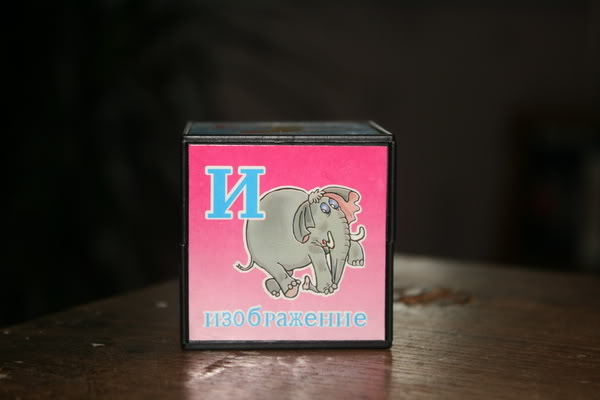
\includegraphics[width = \linewidth]{images/01-test.jpg}
\end{frame}


\framepic{images/01-test.jpg}{\vspace{-0.2cm} \color{colorblue} картинка}

\end{document}